\subsubsection{usergoal-ugSecurelyUseSystem}

\label{RE-use-case-ugSecurelyUseSystem}



the actAdministrator's goal is to follow an identification procedure to be allowed to add or delete the necessary crisis coordinators that will be granted the responsibility to handle alerts and crisis. 


\begin{usecase}
  \addheading{Use-Case Description}
  \addsingletwocolumnrow{Name}{ugSecurelyUseSystem}
  \addsingletwocolumnrow{Scope}{system}
  \addsingletwocolumnrow{Level}{usergoal}
  

\addrowheading{Primary actor(s)}
\addnumberedsinglerow{}{\msrcode{actAuthenticated[active]}}



\addrowheading{Goal(s) description}
\addsinglerow{
the actAdministrator's goal is to follow an identification procedure to be allowed to add or delete the necessary crisis coordinators that will be granted the responsibility to handle alerts and crisis. 
}

\addrowheading{Reuse}
\addnumberedsinglerow{}{\msrucname{oeLogin [1..1]}}
\addnumberedsinglerow{}{\msrucname{oeBioLogin [1..1]}}
\addnumberedsinglerow{}{\msrucname{oeLogout [1..1]}}
\addnumberedsinglerow{}{\msrucname{oeUpdateBio [1..*]}}

\addrowheading{Protocol condition(s)}
\addnumberedsinglerow{}{
the iCrash system has been deployed
}

\addrowheading{Pre-condition(s)}
\addnumberedsinglerow{}{
none
}

\addrowheading{Main post-condition(s)}
\addnumberedsinglerow{}{
the actAuthenticated is known by the system not to be logged.
}

\addrowheading{Main Steps}
\addalphanumberedsinglerow{}{the actor \msrcode{actAuthenticated} executes the \msrucname{oeLogin} use case}
\addalphanumberedsinglerow{}{the actor \msrcode{actAuthenticated} executes the \msrucname{oeBioLogin} use case}
\addalphanumberedsinglerow{}{the actor \msrcode{actAuthenticated} executes the \msrucname{oeUpdateBio} use case}
\addalphanumberedsinglerow{}{the actor \msrcode{actAuthenticated} executes the \msrucname{oeLogout} use case}
\addrowheading{Steps Ordering Constraints}
\addnumberedsinglerow{}{step (a1) or (a2) must always precede step (c).}
\addnumberedsinglerow{}{step (a1) or (a2) must always precede step (b).}
\addnumberedsinglerow{}{step (b) can be executed multiple times.}


\end{usecase} 


Figure \ref{fig:lu.uni.lassy.excalibur.examples.icrash-RE-UCD-uc-ugSecurelyUseSystem}
shows the use case diagram for the ugSecurelyUseSystem user goal use case

\begin{figure}[htbp]
\begin{center}

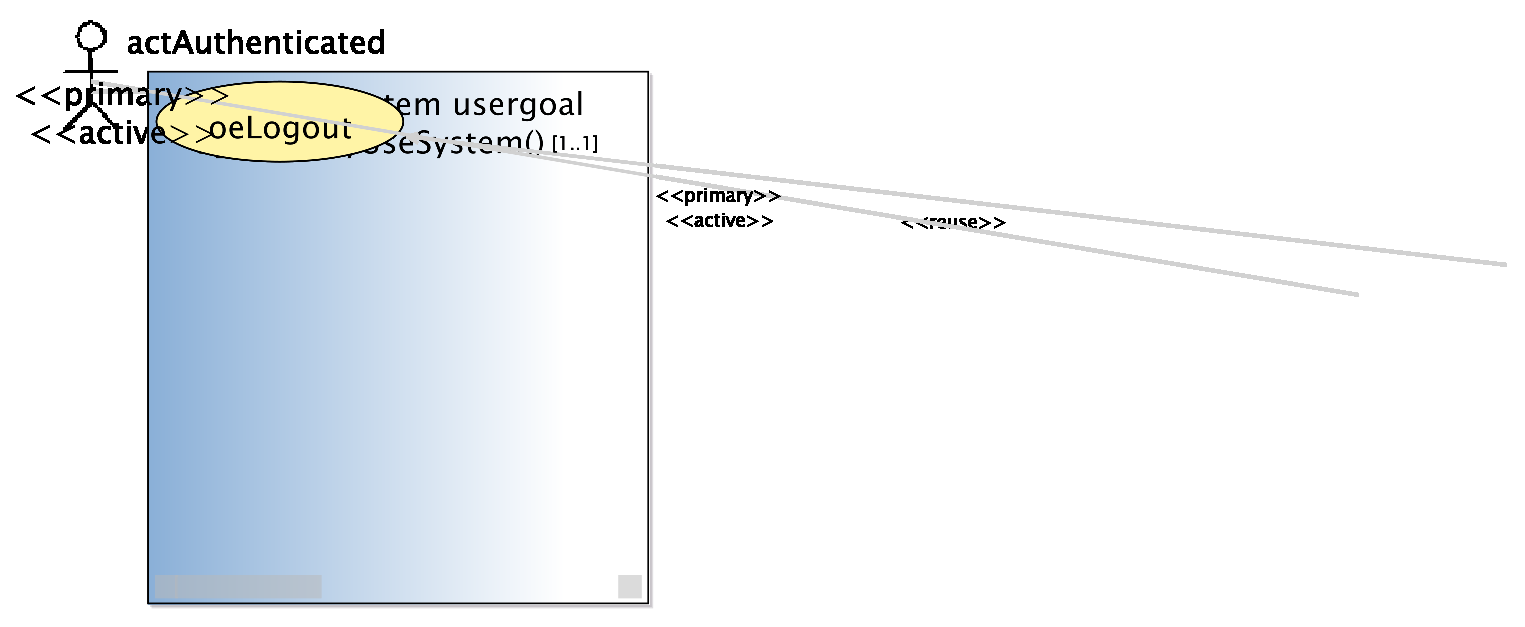
\includegraphics[
angle=0
,scale=0.75
]{./images-report-gen/usecase-model/usergoal/uc-ugSecurelyUseSystem.eps}
\end{center}
\caption[lu.uni.lassy.excalibur.examples.icrash Use Case Diagram: uc-ugSecurelyUseSystem]{ ugSecurelyUseSystem user goal use case}
\label{fig:lu.uni.lassy.excalibur.examples.icrash-RE-UCD-uc-ugSecurelyUseSystem}
\end{figure}
\vspace{0.5cm}
